\documentclass[a4paper,12pt,ngerman]{scrartcl}
\usepackage{babel}
\usepackage{mathptmx}
\usepackage[T1]{fontenc}
\usepackage[utf8x]{inputenc}
\usepackage[a4paper,lmargin=2.5cm,rmargin=2.5cm,tmargin=2.0cm,bmargin=2.0cm,footskip=0.5cm]{geometry}
\usepackage{amsmath}
\usepackage{amssymb}
\usepackage{graphicx}
\usepackage{hyperref}

\addtokomafont{sectionentry}{\normalfont}
\addtokomafont{section}{\normalfont}
\addtokomafont{subsection}{\normalfont}

\graphicspath{ {./images/} }

\renewcommand{\baselinestretch}{1.5} 

\begin{document}
\begin{titlepage}
	Projekttitel: Debuggen mit KI
	\vspace{1cm}
	
	Teilnehmende: PLACEHOLDER
	
	Erarbeitungsort: ?
	
	Projektbetreuende: PLACEHOLDER
	
	Thema des Projekts: Kann eine KI beim Debuggen eines Programms helfen?
	
	Fachgebiet: Informatik
	
	Wettbewerbsparte: Jugend forscht
	
	Bundesland: PLACEHOLDER
	
	Wettbewerbsjahr: 2024
	
	\vspace{2cm}
	\vfill
\end{titlepage}
\clearpage
\tableofcontents
\clearpage

\section{Fachliche Kurzfassung}

Unsere Frage ist es, ob es möglich ist, dass eine KI für einen Programmierer den Debug Prozess übernimmt und selbstständig im Code den Grund für gegebene Fehler finden kann, ähnlich dazu, wie man es als Programmierer tun würde. Hierzu fügen wir eine Middleware in den Debug Prozess von VSCode zwischen Editor und Debug Adapter ein, welcher in der Kommunikation des Debuggers Nachrichten mitlesen, unterbrechen und hinzufügen kann. Ein großes Problem ist, wie die KI mit dieser Middleware kommunizieren wird, da LLMs nur Text Nachrichten empfangen und zurücksenden können. Wir benötigen also eine Konvertierung zwischen dem Debug Adapter Protokoll (DAP) und einem für die KI interpretierbaren und produzierbaren Text.

Um den Debug Prozess auf diese Art und Weise verändern zu können, benutzen wir eine VSCode Extension, die beim Starten des Debug Adapters die Funktionen, die zur Kommunikation benutzt werden, mit eigenen Funktionen ersetzt, welche mit der KI kommunizieren und Nachrichten weiterhin mit den originalen Funktionen an den Editor oder an den Debug Adapter senden können.

Nun müssen die Daten des Debug Adapters (DA) in für die KI verständliche Begriffe übersetzt werden. Hierfür, stellen wir der KI verschiedene Kommandos zum empfangen oder senden zur Verfügung, die von einem Übersetzer in DAP Nachrichten umgewandelt werden. Die KI kann so beispielsweise Breakpoints setzen, das Programm weiterlaufen lassen, oder den Wert einer Variable erfragen. Folgende Kommandos sind für die KI zum Senden verfügbar:
\begin{itemize}
	\item ``BREAKPOINT [Zeile] [Datei]'' (setzen eines Breakpoints)
	\item ``CONTINUE'' (Programm weiterlaufen lassen)
	\item ``STEP'' (Einen Programmschritt ausführen)
	\item ``STEPINTO'' (In einen Funktionsaufruf eintreten)
	\item ``STEPOUT'' (Aus einem Funktionsaufruf austreten)
	\item ``VARIABLE [Name]'' (Variablen auslesen)
	\item ``LINE [Zeile] [Datei]'' (Einzelne Zeilen von Dateien auslesen)
	\item ``ERROR [Fehlermeldung]'' (Wenn die KI, nachdem sie die Anweisungen erhalten hat, irgendetwas vom debuggen abhält)
	\item ``CAUSE [Beschreibung]'' (Wenn schlussendlich der Grund für den Bug gefunden wurde).
\end{itemize}
Außerdem kann die KI folgendes Kommando erhalten:
\begin{itemize}
	\item ``PAUSED [Zeile] [Spalte] [Datei]'' (Wenn das Programm pausiert).
\end{itemize}

Zum Testen dieser KI haben wir sie mit verschiedenen Bugs ausprobiert und jeweils beurteilt, wie hilfreich die Antwort der KI zum Beheben der Bugs war.

TODO: Ergebnisse

Der Code für unser Projekt ist öffentlich auf GitHub verfügbar: \url{https://github.com/Papierkorb2292/AI-Debugger}

\section{Motivation und Fragestellung}

Mit den letzten Fortschritten und dem öffentlichen Zugang zu KI, werden viele Möglichkeiten untersucht, wie eine KI beim Programmieren helfen kann. So gibt es beispielsweise schon länger die Möglichkeit Code Vorschläge von einer KI wie Tabnine oder Github Copilot zu erhalten und mit LLMs, wie ChatGPT, lässt sich auch ein ganzer Codeblock automatisch schreiben.

Wir haben uns gefragt, ob KI Programmierenden auch beim Debuggen von geschriebenen Programmen helfen kann. Die KI ``Devin'' kann bereits selbst Programme schreiben und debuggen, benutzt allerdings zum debuggen \texttt{print} Statements, um den Zustand des Programms zu überwachen, indem dieser Stellenweise in die Textausgabe geschrieben wird. Unser Ziel ist es jedoch die KI mit einem Debug Server, den auch Programmierende in ihrem Editor sonst benutzen, kommunizieren zu lassen. Ein weiterer Vorteil hiervon ist, dass man selbst zusammen mit der KI debuggen kann, indem man die KI nur Teile des Debuggen übernehmen lässt, und man den Rest noch selbst über den Editor vornimmt.

\section{Hintergrund und theoretische Grundlagen}

\subsection{KI}

Als KI (Künstliche Intelligenz) bezeichnet man häufig Verfahren zur Datenverarbeitung, für die keine genaue Handlungsanweisung festgelegt werden, sondern die mit Hilfe von Maschinellen Lernen erstellt wird, was einfach gesagt bedeutet, dass man die Parameter des Verfahrens stückweise ändert, um bei Eingangsdaten, für die schon Ausgangsdaten bekannt sind, die Ausgangsdaten des Verfahrens so nah wie möglich an die Erwarteten zu bekommen$^1$. Oft liegt der KI an neuronales Netzwerk zugrunde, in welchem Eingangsdaten über mehrere Iterationen hinweg verschiedenen gewichtet und addiert werden können, um am Ende auf die Ausgangsdaten zu kommen.

Als LLM (Large Language Model) bezeichnet man KIs, die Textdaten verarbeiten und auf solche trainiert sind$^3$. Ein bekanntes Beispiel ist ChatGPT: Eine KI, welcher der Benutzer Textanfragen schreiben, und die dann selbst eine Textantwort produziert. LLMs zeichnen sich zudem durch ihre Flexibilität aus, da sie viele verschiedene Aufgaben über Text erledigen können und die Möglichkeit haben vielen Fragen zu beantworten$^2$.

\subsection{Debugging}

Beim Debuggen eines Programm mit einem Debugger, verbindet sich der Editor mit einem Debug Server, der das Programm ausführt und das Programm auch pausieren kann, damit der Editor den Zustand des Programms zu einem bestimmten Punkt anzeigen kann. Während das Programm pausiert ist, lässt sich außerdem mit dem Editor Schritt für Schritt durch das Programm durchgehen, um die Änderungen im Zustand des Programms zu beobachten.

\subsection{Debug Adapter}

Weil ein Debug Server direkt mit dem auszuführendem Programm interagiert, ist die Schnittstelle zum Debug Server oft spezifisch zur Sprache des Programms. Um den Editor mit dem Debug Server zu verbinden, wird deshalb ein Debug Server Adapter benutzt, der spezifisch zu einem Debug Server ist, und für welchen die Kommunikation mit dem Editor von Microsoft auf das Debug Adapter Protokoll (DAP) festgelegt wurde. Für jeden Debug Server kann so auch ein Debug Adapter angeboten werden, der mit dem Debug Server kommunizieren kann$^4$.

Folgendes ist eine Veranschaulichung, wie der Debug Prozess also aufgebaut ist:

\begin{center}
	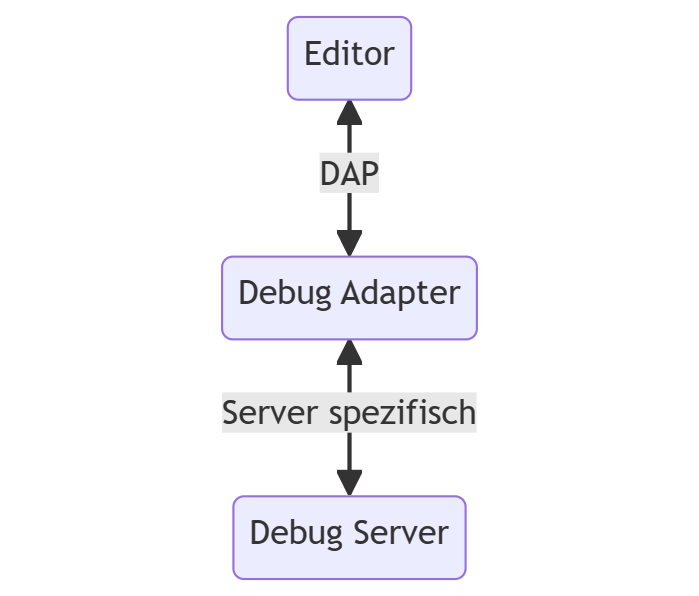
\includegraphics[width=0.5\textwidth]{debugger}
\end{center}

\section{Vorgehensweise, Materialien und Methoden}

Um zu testen, ob es möglich ist, eine KI auf diese Art und Weise beim Debuggen unterstützen zu lassen, werden wir selbst unsere Idee hierzu umsetzen, und verschiedene Ansätze, um mit der KI zu interagieren, auszuprobieren.

Um eine KI in den Debug Prozess zu interagieren, fügen wir zunächst eine Middleware zwischen Editor und Debug Adapter hinzu, durch welche alle Nachrichten zwischen dem Editor und Debug Adapter laufen, damit die KI diese beobachten und unterbrechen kann. Außerdem wird es hiermit möglich, Nachrichten, die durch die KI eingebracht werden, an den Editor und Debug Adapter zu senden. Dies macht es möglich für die KI Kontrolle über den Debug Prozess zu nehmen.

Es gibt verschiedene Möglichkeiten, wie die KI selbst laufen kann. Zunächst werden wir von OpenAI das KI Modell GPT-4o benutzen, mit welchem man über das Internet kommuniziert. Es wäre außerdem möglich später verschiedene KI Modelle auszuprobieren, um zu testen, wie gut verschiedene Modelle debuggen können.

\subsection{KI Debugger Dienst}

Der wichtigste Teil, ist allerdings, wie die KI mit ihren Nachrichten mit dem Benutzer, dem Editor und dem Debug Adapter kommuniziert. Der Benutzer muss nämlich die Möglichkeiten haben Nachrichten an die KI zu senden, die KI muss antworten können, und zusätzlich muss eine Übersetzung zwischen DAP Nachrichten (normalerweise werden diese zwischen Editor und Debug Adapter gesendet) und dem Text, über welchen die KI kommuniziert, stattfinden. Im folgenden wird dieser Teil als ``KI Debugger Dienst'' betitelt. Außerdem muss der Editor den Kontext, also beispielsweise den Inhalt der Dateien, in denen gedebuggt wird, an den KI Debugger Dienst senden, damit dieser weiß, welche Positionen in den Dateien den verschiedenen Teilen des laufenden Programms entsprechen, um an diesen Stellen pausieren zu können.

Folgendes Diagramm veranschaulicht nochmal den erweiterten Aufbau des Debuggers zusammen mit der Kommunikation mit der KI.

\begin{center}	
	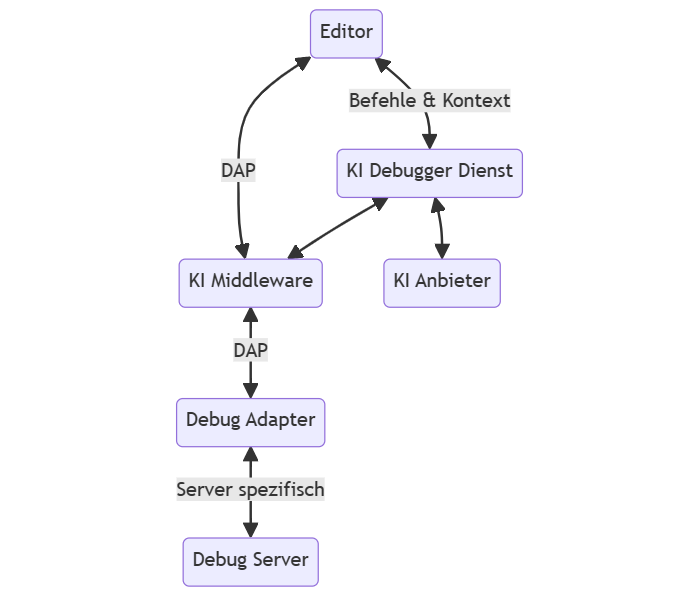
\includegraphics[width=0.5\textwidth]{ai_integration}
\end{center}

Um zu verstehen, wie die Kommunikation zwischen dem Debug Adapter (DA) und dem KI-Debugger-Dienst (KDD) funktioniert, müssen deren Verarbeitung und Komprimierung genauer betrachtet werden.

Da DAP Nachrichten im JSON Format gesendet werden und dabei oft viele Informationen über den Zustand des Programms enthalten, bei denen wichtig ist, dass sie akkurat sind, wie Dateipfade, Breakpoint Ids, etc., haben wir uns dagagen entschieden, die KI direkt diese JSON Objekte lesen und auslesen zu lassen, da dann die KI viel mehr Wert darauf legen müsste, vollständig fehlerfreie JSON Objekte auszugeben, was die Qualität des Debuggens vermindern könnte.

Stattdessen kommuniziert die KI mit dem KI Debugger Dienst über simple Textnachrichten, von denen jede ein Kommando darstellt. So ein Kommando ist aufgebaut aus einem Kommando Namen und einer Liste von Argumenten, die das Kommando benötigt. Beispielsweise gibt es das Kommando ``BREAKPOINT [Zeile] [Datei]'', welches der KI erlaubt einen Breakpoint in einer bestimmten Datei und Zeile zu setzen, was bedeutet, dass das Programm pausiert, wenn es diese Zeile erreicht. Über die gleiche Art und Weise werden auch bestimmte Events der KI mitgeteilt, indem die KI beispielsweise das Kommando ``PAUSED [Zeile] [Spalte] [Datei]'' erhält, sobald das Programm pausiert.

Alle der KI zur Verfügung stehenden Kommandos werden ihr in der ersten Nachricht mitgeteilt, zusammen mit ihrem Sinn als Debugger und dem zu behebenden Bug. Das Vermitteln der Kommandos geschieht hierbei durch festgelegte Sätze, also werden diese Kommandos in eine sprachliche Form gebracht, die die Kommunikation mit dem LLM (Large Language Model) ermöglicht. Beispielsweise entspricht das Kommando ``BREAKPOINT'' dem Satz: ``You can set breakpoints in the code by starting your message with "BREAKPOINT" followed by the line number and the file name.'' Dieses Prinzip wird auf jedes Kommando angewendet. Nun, da die Befehle für die KI vorliegen, werden diese übermittelt und die Antworten empfangen. Die jeweiligen Antworten sind so formatiert, dass sie ohne großen Aufwand weiterverarbeitet werden können.

Da wir davon ausgehen, dass die KI nicht immer die Fragestellung ausreichend verstehen wird, haben wir ihr außerdem die Möglichkeit gegeben, Fehler auszugeben, indem sie das Kommando ``ERROR [Fehlermeldung]'' sendet. Dieses Kommando wird an den Editor weitergeleitet, sodass ein User die Fehlermeldung sehen kann und die Anfrage anpassen kann.

Wie bereits erwähnt ist es außerdem wichtig, dass die KI Zugriff auf den Code des Programs bekommt. Auch hierfür gibt es ein Kommando, welches eine Zeile aus einer Datei zu der KI senden kann, wenn die KI ``LINE [Zeile] [Datei]'' sendet. Hierbei meiden wir, eine gesamte Datei auf einmal an die KI zu senden, da dies darfür sorgen könnte, dass die KI sich nicht den genauen Inhalt der einzelnen Zeilen richtig merken kann. Außerdem würde, wenn man der KI eine ganze Datei senden würde, dies viele Tokens verbrauchen, was schlussendlich dafür sorgt, dass der Debug Prozess mehr kostet.

\subsection{Einbinden der KI}

Dieses Kommando System muss nun in den Debug Prozess eingebunden werden, da im Moment noch das Erhalten und Senden von Kommandos unabhängig vom Debuggen passiert. Hierfür haben wir der KI zusätzlich folgende Kommandos zur Verfügung gestellt, mit Hilfe derer sie ähnlich wie der User mit dem Debug Prozess interagieren kann: ``CONTINUE'', ``STEP'', ``STEPINTO'', ``STEPOUT''. Jeder dieser Kommandos entspricht einem Knopf im Editor, den der Benutzer drücken kann, um das Programm weiterlaufen zu lassen, oder um Schritt für Schritt durch das Programm zu gehen. Wenn die KI ein solches Kommando sendet, wird eine entsprechende DAP Nachricht an den Debug Adapter gesendet, während außerdem eine Nachricht an den Editor gesendet wird, die diesem sagt, der Debug Adapter wäre von alleine weitergelaufen, sodass der User den Verlauf des Debuggens mitverfolgen kann.

Während in Folge eines dieser Kommandos das Program weiterläuft, bis es am nächsten Breakpoint angekommen ist oder den angeforderten Schritt ausgeführt hat, wird hingegen die Konversation mit der KI pausiert. Diese geht erst weiter, wenn das Programm wieder pausiert hat, woraufhin die bereits genannte ``PAUSED'' Nachricht an die KI gesendet wird. Auf diese Art und Weise erhalten wir eine Art Rückkopplung, die abwechselnd den Debug Prozess oder die KI laufen lässt und so der KI das schritthafte Debuggen ermöglicht.

Ein weiteres wichtiges Kommando ist ``VARIABLE [Name]'', welches der KI erlaubt den Wert einer Variable zu erfragen, sodass die KI den Zustand des Programms aktiv verfolgen kann und dadurch direkt Rückschlüsse darauf ziehen kann, an welcher Stelle im Code der Zustand vom erwarteten Zustand abweicht.

Zuletzt hat die KI außerdem ein ``CAUSE [Beschreibung]'' Kommando, mit dem sie zum Abschluss den von ihr herausgefunden Grund ausgeben kann, warum der Bug aufgetreten ist.

\subsection{Komprimierung der Konversation}

Ein weiterer wichtiger Aspekt ist die Komprimierung der übermittelten Daten. Dies ist aufgrund des Bezahlmodells von OpenAI wichtig, das nach dem Prinzip 'You pay w

\subsection{Erheben von Daten}

Da nun die KI in den Debug Prozess integriert wurde, ist der nächste Schritt die Fähigkeiten der KI auszutesten, um herauszufinden, ob sie tatsächlich in der Lage ist, ein Programm erfolgreich zu debuggen. Hierfür haben wir uns entschieden, die KI auf verschiedene Probleme zu testen, die wir selbst in Programmen eingebaut haben, und die KI dabei zu beobachten, wie sie diese Probleme löst.

Hierbei können wir für jedes Problem beurteilen, wie präzise und für den User verständlich sowie hilfreich die KI den Grund für das Problem formulieren kann. Außerdem können wir beurteilen, wie sehr sie es geschafft hat den zugrundeliegenden Fehler zu erkennen, oder ob es ihr auschließlich gelang einen Folgefehler zu erkennen.

\section{Ergebnisse}

TODO: Ausformulieren
Aufgekommene Probleme:
- KI kann manchmal Probleme haben, die eigene Rolle zu verstehen
- KI liest manchmal nicht genug Zeilen ein

- Funktioniert aber sonst gut :D

\section{Ergebnissdiskussion}

\section{Fazit und Ausblick}

\subsection{Ausblick}

Wir denken, dass sich wesentlich bessere Ergebnisse erzielen lassen würden, wenn man anstatt einer allgemeinen KI, die auf viele verschiedene Aufgaben trainiert ist, eine spezifische KI für das Debuggen trainiert. Es wäre beispielsweise möglich, diese KI auch auf die Syntax von Programmiersprachen spezialisiert zu trainieren, sodass sie das Program und die Aufgabe besser versteht.

Um so eine KI zu trainieren, wäre es möglich die Middleware bei normalen Debug Prozessen mitlaufen zu lassen, sodass die Kommunikation zwischen Editor und Debug Adapter aufgezeichnet wird. Das würde es erlauben die KI auf die aufgezeichneten Daten zu trainieren, sodass sie lernt den Editor und daher auch die Programmierenden nachzustellen. Fraglich ist, ob es möglich wäre von den aufgezeichneten Daten auf das Problem und die Problemlösung zu schließen, oder ob es notwendig wäre, dass die Programmierenden, wenn sie ihre Debug Prozesse aufzeichnen möchten, auch zusätzliche Informationen über das Problem und die anschließend angewandte Lösung angeben müssten, sodass die KI lernen würde das Problem einzulesen und die Lösung auszugeben.

Eine weitere Verbesserungsmöglichkeit wäre dem bereits von uns erstelltem System mehr Kommandos hinzuzufügen, um der KI mehr Kontrolle über den Debug Prozess zu geben. Beispielweise könnte man es der KI möglich machen eine Liste aller Variablen zu erhalten, den Call stack auszulesen, also die Reihenfolge der Funktionsaufrufe zu erhalten, oder auch die Möglichkeit geben, den Wert einer Variable zu ändern. Dies sind Aktionen, die auch beim normalen Debuggen oft nützlich sind, und die es der KI ermöglichen würden, das Programm besser zu debuggen.

\section{Quellen- und Literaturverzeichnis}

Wikimedia Foundation Inc.,  ``Künstliche Intelligenz - Wikipedia'', grundlegende Information zu künstlicher Intelligenz\\
\url{https://de.wikipedia.org/wiki/K\%C3\%BCnstliche_Intelligenz}, besucht am 19.03.2024\\
Wikimedia Foundation Inc.,  ``Large language model - Wikipedia'', grundlegende Information zu Large Language Models\\
\url{https://en.wikipedia.org/wiki/Large_language_model}, besucht am 19.03.2024\\
Wikimedia Foundation Inc.,  ``Language model - Wikipedia'', grundlegende Information zu Language Models \\
\url{https://en.wikipedia.org/wiki/Language_model}, besucht am 19.03.2024\\
Microsoft, ``Overview [über das Debug Adapter Protokol]'', grundlegende Information zum Debug Adapter Protokoll
\url{https://microsoft.github.io/debug-adapter-protocol/overview.html}, besucht am 25.03.2024\\
\vspace{1em}\\
Microsoft, ``Extension API | Visual Studio Code Extension API'', Anleitung zum Entwickeln einer VSCode Extension\\
\url{https://code.visualstudio.com/api}, besucht am 19.03.2024\\
Microsoft, ``vscode/blob/main/src/vs/workbench/contrib/debug/node/debugAdapter.ts at main microsoft/vscode'', VSCode Quellcode zur Kommunikation mit Debug Adaptern\\
\url{https://github.com/microsoft/vscode/blob/main/src/vs/workbench/contrib/debug/node/debugAdapter.ts}, besucht am 19.03.2024

\end{document}